\section{Мета роботи}
Набути досвіду практичної роботи розв’язання задач з використанням бінарних дерев.

\noindent
\textbf{Теми для попередньої роботи:}
\begin{itemize}
    \item балансування дерев;
    \item АВЛ-дерева;
    \item червоно-чорні дерева;
    \item дерева Хаффмана;
    \item дерева для арифметичних виразів.
\end{itemize}


\section{Завдання}
Розробити програму, що створює бінарне дерево та розв’язує
індивідуальне завдання. Видати вміст дерева та результати індивідуального
завдання на екран.

Побудувати червоно-чорне дерево. Визначити висоту дерева.
Додати вузол із ключем, значення якого визначено висотою дерева.

\section{Хід виконання}
Для виконання завдання було обрано мову Rust.
Увесь код також додатково був розміщений в GitHub репозитарії: \href{https://github.com/blackgolyb/algos-labs}{https://github.com/blackgolyb/algos-labs}.


\newpage
\subsection{Червоно-чорне дерево}
\subsubsection{Node}
Для початку почнемо з розробки вузла нашого дерева також будемо будувати наше дередо за принципом ключ-значення.
Тобто за впорядкування вузлів будуть відповідати саме ключі, а значення будуть просто зберігатися там.
\lstinputlisting[language=Rust, style=colouredRust]{\codeDirectory/src/libs/rb_tree/node.rs}

\subsubsection{RBTree}
\lstinputlisting[language=Rust, style=colouredRust]{\codeDirectory/src/libs/rb_tree/lib.rs}

\subsubsection{Форматуання дерева}
Для нашого дерева також імплементуємо інтерфейс виводу на екран,
щоб було зручно ливитися його вміст.
Будемо виводити тільки ключ, щоб не накладати обмеження на зберігаїмий тип.
\lstinputlisting[language=Rust, style=colouredRust]{\codeDirectory/src/libs/rb_tree/format.rs}


\newpage
\subsection{Приклад роботи програми}
\noindent
Код програми для перевірки:
\lstinputlisting[language=Rust, style=colouredRust]{\codeDirectory/src/labs/lab14/main.rs}

\begin{figure}[ht!]
    \centering
    \subfigure[]{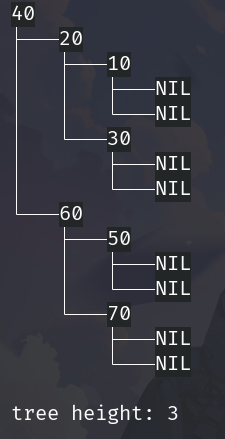
\includegraphics[height=10cm]{\assetsDirectory/res1.png}}
    \subfigure[]{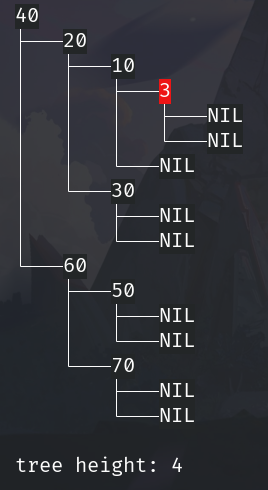
\includegraphics[height=10cm]{\assetsDirectory/res2.png}}
    \caption{Приклад роботи програми  (а) до додавання вузла (б) після додавання вузла}
\end{figure}


\newpage
\section{Висновки}
В ході виконання лабораторної робити було створено червоно-чорне дерево та функції роботи з ним.
